\documentclass{article}
\usepackage[utf8]{inputenc}
\usepackage[T1]{fontenc}
\usepackage{amsmath}
\usepackage{hyperref}
\usepackage{graphicx}
\usepackage{url}
\usepackage{subfigure}

\newcommand{\code}{\texttt}

\title{Project in Information-Theoretic Modeling Final Report}
\author{Aleksi Hartikainen \and Mikko Sysikaski}

\begin{document}
\maketitle

%\abstract{}

%\newpage
%\tableofcontents
%\newpage

\section*{Problem 1}

The first task was to compress a sequence of bits using side data that was also available during decompression.

The file to be compressed had $100\,000$ binary digits, so trivially packing the bits yields a file of size $12\,500$ bytes.
For comparison, we also tried packing the data this way as the decompression code becomes much smaller and simpler.
This gave a total size of around 13.5~KiB uncompressed, and 12.5~KiB after compressing with gzip.

The task was to use arithmetic coding with probabilities from the given model.
Instead of using probabilities from model definition, we computed actual conditional frequencies from the data.
That is, for every tuple $(x_1,x_2,x_3,x_4)$ we counted how many times $x_0$ is 0 and 1, and this gave us the conditional probability of $x_0$ with respect to the other variables.
The calculated probabilities are shown in Figure~\ref{ex1_probs}.
We created a custom implementation of arithmetic coding that used the conditional probabilities of Figure~\ref{ex1_probs} to encode each bit.

Using arithmetic coding and the conditional probabilities, we got the data compressed in 8100~bytes.
Together with the decompression program, this gave a total file size of 9832~bytes.

To evaluate the correctness of our arithmetic coding implementation, we calculated also the theoretical bound for data size using entropy coding.
According to probabilities in Figure~\ref{ex1_probs}, the total entropy of the input file is 64790.4~bits, which is 8098.8~bytes, so the result generated by our implementation is within 1 byte of the theoretical optimum.


\begin{figure}
\label{ex1_probs}

\begin{center}
\begin{tabular}{|c|c|c|c|c|c|}
\hline
$x_1$ & $x_2$ & $x_3$ & $x_4$ & $P(x_0 = 0)$ & $P(x_0 = 1) $ \\ \hline
   0 & 0 & 0 & 0 & 0.74244 & 0.25756 \\ \hline
   1 & 0 & 0 & 0 & 0.180631 & 0.819369 \\ \hline
   0 & 1 & 0 & 0 & 0.122035 & 0.877965 \\ \hline
   1 & 1 & 0 & 0 & 0.595336 & 0.404664 \\ \hline
   0 & 0 & 1 & 0 & 0.507643 & 0.492357 \\ \hline
   1 & 0 & 1 & 0 & 0.072675 & 0.927325 \\ \hline
   0 & 1 & 1 & 0 & 0.0461351 & 0.953865 \\ \hline
   1 & 1 & 1 & 0 & 0.359641 & 0.640359 \\ \hline
   0 & 0 & 0 & 1 & 0.888336 & 0.111664 \\ \hline
   1 & 0 & 0 & 1 & 0.37004 & 0.62996 \\ \hline
   0 & 1 & 0 & 1 & 0.277587 & 0.722413 \\ \hline
   1 & 1 & 0 & 1 & 0.78809 & 0.21191 \\ \hline
   0 & 0 & 1 & 1 & 0.733648 & 0.266352 \\ \hline
   1 & 0 & 1 & 1 & 0.177577 & 0.822423 \\ \hline
   0 & 1 & 1 & 1 & 0.119161 & 0.880839 \\ \hline
   1 & 1 & 1 & 1 & 0.582299 & 0.417701 \\ \hline
\end{tabular}
\end{center}
\caption{Conditional probabilities used in exercise 1}
\end{figure}

\section*{Problem 2}

The second task was to compress data consisting of stock prices of four different stocks. The data consisted of floating point values with two decimals. As we didn't want to think about floating point accuracy issues, we simply converted the initial data to integers by multiplying the values by 100 and divided our final result again by 100 before outputting it.

To find a good compression scheme, we initially tried plotting the data, as shown in Figure~\ref{fig:ex2o}.
As there was no immedient regularity to be seen, we tried seeing how the values change by taking the differences of adjacent values, shown in Figure~\ref{fig:ex2d}.
It can be seen that there are some large negative peaks, but otherwise the differences stay close to zero.
The same behavior can be observed for each of the stocks.

\begin{figure}
	\subfigure[Original data]{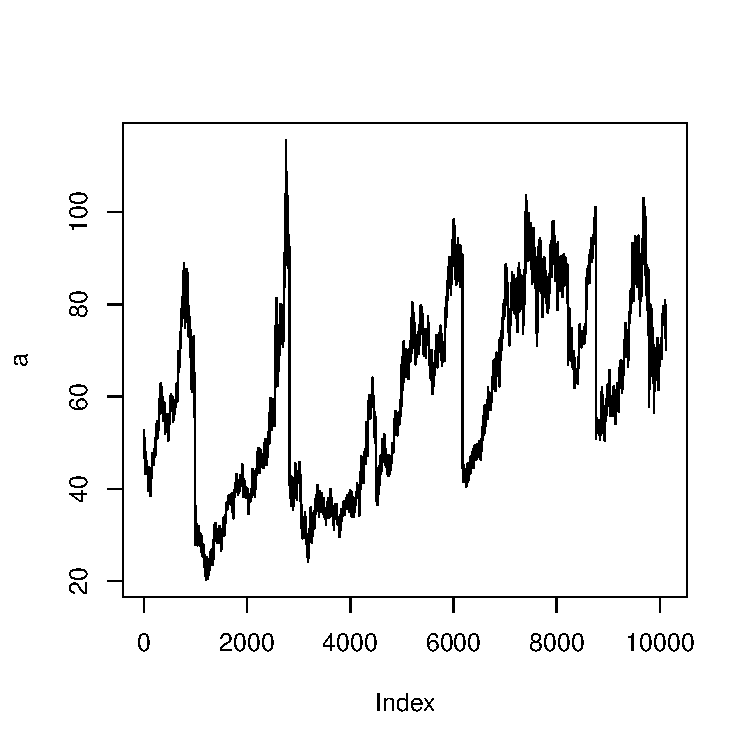
\includegraphics[scale=0.5]{ex2_orig.pdf}\label{fig:ex2o}}
	\subfigure[Differences of consecutive values]{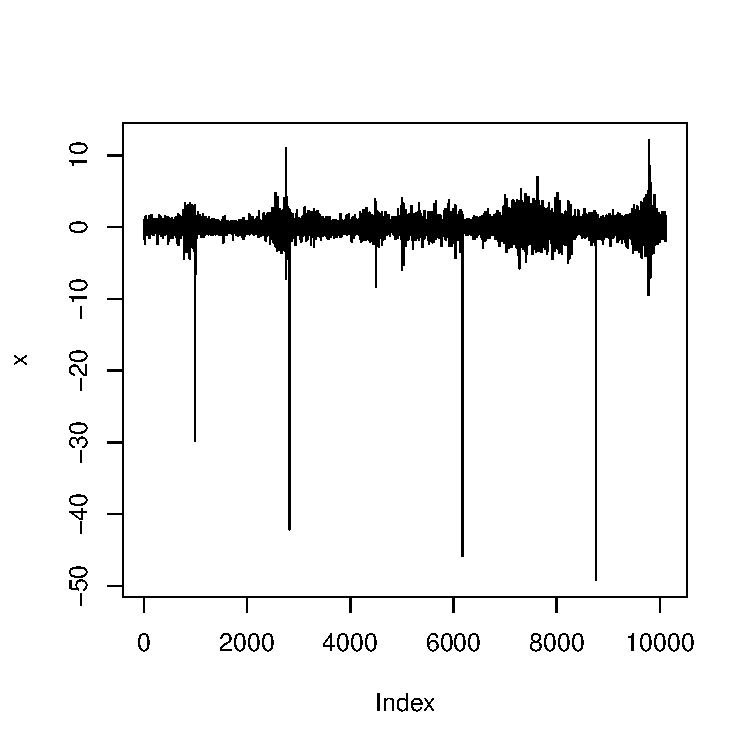
\includegraphics[scale=0.5]{ex2_diff.pdf}\label{fig:ex2d}}
	\caption{Plot of the first column of the data and the differences between its consecutive values. The original data shows a lot of irregularities, but except for a few peaks, the changes between consecutive values are quite small.}
\end{figure}

The connection between the four stocks changes didn't seem very simple so we decided to try simply compressing each of the stocks separately.
As our tests suggested that the differences between adjacent values are close to zero, we used a simple Gaussian model with mean equal to the previous value to calculate the probabilities for each value that where used in the arithmetic coding.

It seemed that the variance of the values varied quite a lot over time, so we used an adaptive scheme to decide the variance used by the normal distribution to compress each value.
The scheme works by maintaining a current approximation of variance $v_n$ and calculating new approximation $v_{n+1}$ each time we process a new value $x_{n+1}$.
The approximation is updated using the formula $v_{n+1} = \frac{Lv_n + (x_{n+1}-x_n)^2}{L+1}$, where $L$ is a constant that decides how quickly the value changes.
We experimented with different values and saw that picking $L=10$ gives generally good results.

The Gaussian model with adaptive variance had a problem that the probability of the peaks is extremely low, around $10^{-100}$.
As our arithmetic coding uses 32-bit integers, it is impossible to cope with probabilities smaller than $2^{-30}$.
To fix this, we added a constant $2^{-30}$ to probabilities of all values and scaled the normal distribution probabilities so that the total probability still sums to 0.
As the largest number in the data (after converting to integers) was 45100, we only needed to add the constant to first 45101 integers, and scale the original probabilities by $\frac{2^{30}-45101}{2^{30}} \approx 0.999953$.
This factor is so close to 1 that it doesn't hinder the overall compression quality much, while adding the constant guarantees that any value can be encoded using no more than 30 bits.

\section{Optimizing the executable size}

As the goal was to minimize total package size, we decided to use C to have as small binary size as possible.
On linux linking to the standard library increases binary size quite a lot, so we avoided using it and implemented input and output in Assembly with system calls instead.

%\bibliographystyle{abbrv}\bibliography{ref}

%\appendix

\end{document}
